In this section, the NRML schema for the \gls{vulnerability model} is
described in detail. In order to do so, a graphical representation of a
\gls{vulnerability model} (mean loss ratio for a set of intensity measure
levels) is illustrated in Figure~\ref{fig:vulnerability-zero-cov}.

\begin{figure}[ht]
\centering
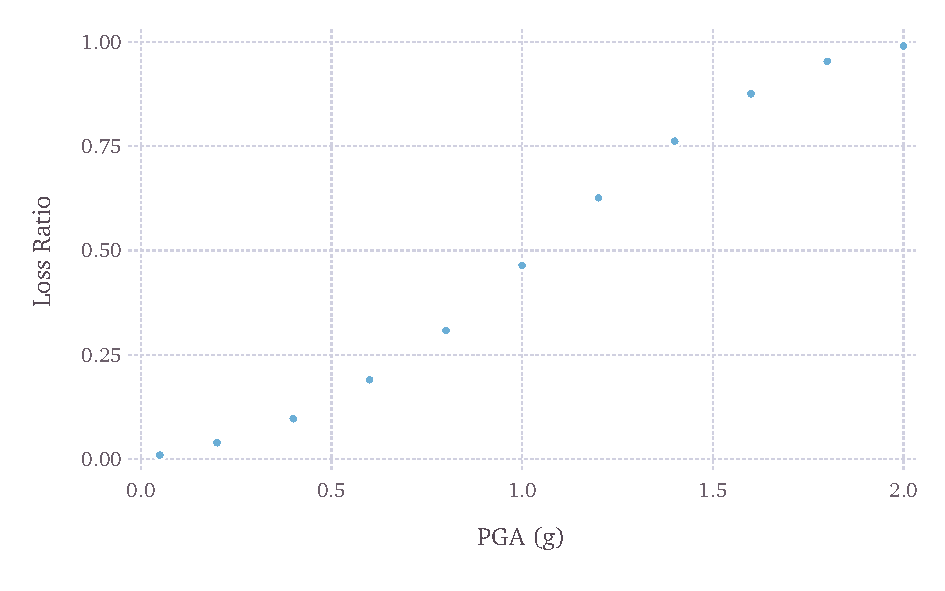
\includegraphics[width=12cm]{figures/risk/vulnerability-zero-cov.pdf}
\caption{Graphical representation of a vulnerability model.}
\label{fig:vulnerability-zero-cov}
\end{figure}

Note that although the uncertainty for each loss ratio is not represented in
Figure~\ref{fig:vulnerability-zero-cov}, it can be considered in the input
NRML file, by means of a coefficient of variation per loss ratio and a
probabilistic distribution, which can currently be set to lognormal (LN) or
Beta (BT). An example of a \gls{vulnerability function} that models the 
uncertainty in the loss ratio at different intensity levels using a lognormal
distribution is illustrated below in Figure~\ref{fig:vulnerability-nonzero-cov}.

\begin{figure}[ht]
\centering
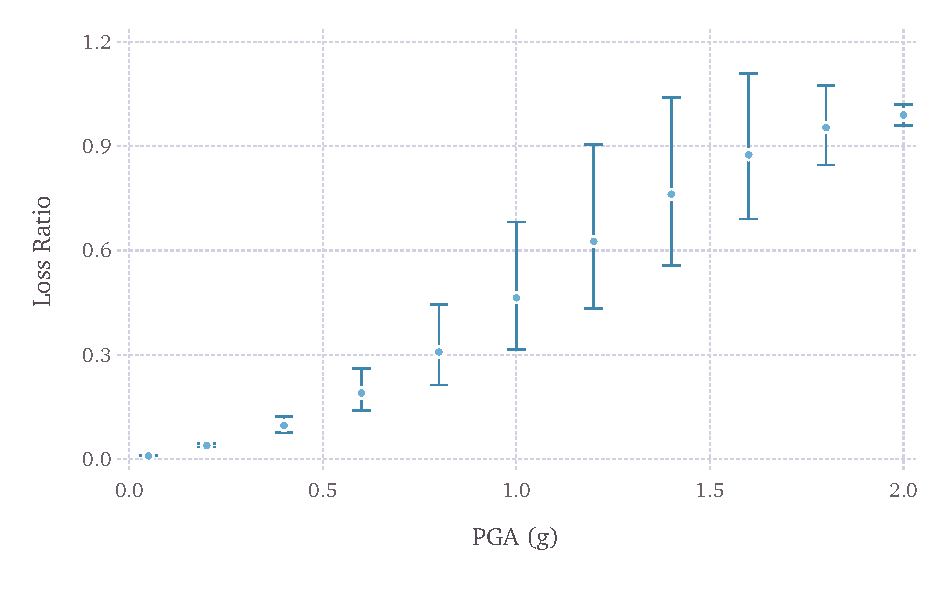
\includegraphics[width=12cm]{figures/risk/vulnerability-nonzero-cov.pdf}
\caption{Graphical representation of a vulnerability function that models the uncertainty in the loss ratio using a lognormal distribution. The mean loss ratios and coefficients of variation are illustrated for a set of intensity levels.}
\label{fig:vulnerability-nonzero-cov}
\end{figure}


An example \gls{vulnerability model} comprising three \glspl{vulnerability
function} is shown below. This \gls{vulnerability model} contains one function
that uses the lognormal distribution to represent the uncertainty in the loss
ratio at different intensity levels, one function that uses the Beta
distribution, and one function that is defined using a discrete probability
mass distribution.

\inputminted[firstline=1,firstnumber=1,fontsize=\footnotesize,frame=single,linenos,bgcolor=lightgray]{xml}{oqum/risk/Verbatim/input_vulnerability.xml}\\


The initial portion of the schema contains general information that describes
some general aspects of the \gls{vulnerability model}. The information in this
metadata section is common to all of the functions in the \gls{vulnerability
model} and needs to be included at the beginning of every \gls{vulnerability
model} file. The parameters are described below:

\begin{itemize}

    \item \Verb+id+: a unique key used to identify the \gls{vulnerability model}

    \item \Verb+assetCategory+: an optional string used to specify the type of
    \glspl{asset} for which \glspl{vulnerability function} will be defined in this file 
    (e.g: buildings, lifelines)

    \item \Verb+lossCategory+: valid strings for this attribute are 
    ``structural'', ``nonstructural'', ``contents'',  
    ``business\_interruption'', and ``occupants''

    \item \Verb+description+: a brief string with further information about the
    \gls{vulnerability model}, for example, which building typologies are 
    covered or the source of the functions in the \gls{vulnerability model}

\end{itemize}

\inputminted[firstline=4,firstnumber=4,lastline=8,fontsize=\footnotesize,frame=single,linenos,bgcolor=lightgray]{xml}{oqum/risk/Verbatim/input_vulnerability.xml}\\


In order to perform probabilistic or scenario risk calculations, it is
necessary to define a \gls{vulnerability function} for each building typology
present in the exposure model. The \glspl{vulnerability function} require the
user to specify the distribution of the loss ratio for a set of intensity
levels. The loss ratio distributions can be defined using either a discrete or
a continuous format, and the \gls{vulnerability model} file can include a mix
of both types of \glspl{vulnerability function}. It is also possible to define
a vulnerability function using a set of deterministic loss ratios
corresponding to a set of intensity levels (i.e., ignoring the uncertainty in
the conditional loss ratios).

The following snippet from the above \gls{vulnerability model} example file defines
a \gls{vulnerability function} modelling the uncertainty in the conditional loss
ratios using a (continuous) lognormal distribution:

\inputminted[firstline=10,firstnumber=10,lastline=14,fontsize=\footnotesize,frame=single,linenos,bgcolor=lightgray]{xml}{oqum/risk/Verbatim/input_vulnerability.xml}\\

The following attributes are needed to define a \gls{vulnerability function} which
uses a continuous distribution to model the uncertainty in the conditional
loss ratios:

\begin{itemize}

    \item \Verb+id+: a unique key used to identify the \gls{taxonomy} for 
    which the function is being defined. This key is used to relate the 
    \gls{vulnerability function} with the relevant \gls{asset} in the 
    \gls{exposure model}.

    \item \Verb+dist+: for vulnerability function which use a continuous 
    distribution to model the uncertainty in the conditional loss ratios, 
    this attribute should be set to either ``\Verb+LN+'' if using the lognormal
    distribution, or to ``\Verb+BT+'' if using the Beta distribution.

    \item \Verb+imls+: this attribute specifies the list of intensity levels
    for which the parameters of the conditional loss ratio distributions will
    be defined. In addition, it is also necessary to define the intensity 
    measure type (\Verb+imt+).

    \item \Verb+meanLRs+: this field is used to define the mean loss ratios
    for this \gls{vulnerability function} for each of the intensity levels
    defined by the attribute \Verb+imls+. The number of mean loss ratios
    defined by the \Verb+meanLRs+ attribute must be equal to the number of
    intensity levels defined by the attribute \Verb+imls+.

    \item \Verb+covLRs+: this field is used to define the coefficient of 
    variation for the conditional distribution of the loss ratios for this
    \gls{vulnerability function} for each of the intensity levels defined by
    the attribute \Verb+imls+. The number of coefficients of variation of loss
    ratios defined by the \Verb+covLRs+ attribute must be equal to the number
    of intensity levels defined by the attribute \Verb+imls+. The uncertainty
    in the conditional loss ratios can be ignored by setting all of the
    \Verb+covLRs+ for a given \gls{vulnerability function} to zero.

\end{itemize}

Several methodologies to derive \glspl{vulnerability function} are currently being
evaluated by \gls{acr:gem} and have been included as part of the Risk
Modeller's Toolkit, the code for which can be found on a public repository at
GitHub at the following address
\href{http://github.com/gemsciencetools/rmtk}{http://github.com/gemsciencetools/rmtk}.

Scripts to convert \glspl{vulnerability function} in CSV format or as Excel or
ASCII files into NRML are also under development, and can be found at the
OpenQuake platform at the following address:
\href{https://platform.openquake.org/ript/}{https://platform.openquake.org/ript/}.
